\documentclass[
article,
12pt,				% tamanho da fonte
%openright,			% capítulos começam em pág ímpar (insere página vazia caso preciso)
oneside,			% para impressão no anverso. Oposto a twoside
a4paper,			% tamanho do papel. 
chapter=TITLE,		% títulos de capítulos convertidos em letras maiúsculas
section=TITLE,		% títulos de seções convertidos em letras maiúsculas
%subsection=TITLE,	% títulos de subseções convertidos em letras maiúsculas
%subsubsection=TITLE,% títulos de subsubseções convertidos em letras maiúsculas
% -- opções do pacote babel --
english,			% idioma adicional para hifenização
brazil				% o último idioma é o principal do documento
]{abntex2}
\usepackage{TCC_Renda/configs/style} % personalização da ABNTEX2 

\addbibresource{TCC_Renda/pos_textual/referencias.bib} % Seus arquivos de referências

%---------------------------------------------------------------------------------------------
%--------- DADOS BÁSICOS DO TCC (Preencher todos) -------------------------------------
%---------------------------------------------------------------------------------------------
%Substituir 'Nome completo do autor' pelo seu nome e da sua dupla se houver.
\autor{David de Oliveira Rafael Reis Alves} 

% FIXME Substituir 'Título do trabalho' pelo título da trabalho.
\titulo{Demonstrativo automatizado para declaração do imposto de renda com renda variável.}
% Substituir 'Subtítulo (se houver)' pelo subtítulo da trabalho. 
% Se não houver subtítulo, basta deletar o texto.
\subtitulo{}
% Substituir 'Orientador' pelo nome do seu orientador.
\orientador{Mestre.Alciomar Hollanda}
% Se for orientado por uma mulher, comente a linha acima e descomente a linha a seguir.
% \orientador[Orientadora]{Orientadora, Dra.}
% Substituir 'XXXXXX' pelo nome do seu  coorientador. Caso não tenha coorientador, comente a linha a seguir.
\coorientador{}
% Se for coorientado por uma mulher, comente a linha acima e descomente a linha a seguir.
% \coorientador[Coorientadora]{Coorientadora, Dra.}
\dia{10}
\mes{11}
\ano{2022}
\local{Hortolandia-SP}
\formacao{Engenharia da computação}
% Se for mulher, comente a linha acima e descomente a linha a seguir.
%\formacao{Engenheira da Computação}
\bancaa{Mestre. Alciomar Hollanda} %Primeiro membro da banca (normalmente o orientador).
\bancab{} %Segundo membro da banca

%Resumo e palavras-chave do trabalho

%---------Modelo de resumo-------------
%           Contexto
%          Lacuna (Gap)
%           Propósito
%          Metodologia
%           Resultados
%           Conclusões
%--------------------------------------
%Contexto
\resumotcc{ Se a pessoa realizou operações envolvendo ações ou fundos imobiliários na bolsa de valores, ela obrigatoriamente precisa fazer a sua declaração de imposto, de acordo com as regras da receita federal.  
%Gap
 Com isso tem-se a grande possibilidade que esses valores possam ser adulterados de forma involuntária. Levando em conta que essas regras não são de conhecimento geral do publico, gerando confusão na apuracão dos resultados, por se tratarem de valores específicos e que por sua vez precisam ser calculados de forma detalhada para que não haja erros.
%Propósito 
Por meio de \textit{datamining} e bibliotecas disponibilizadas pela ferramenta Python, que por sua vez é uma linguagem dinâmica e de simples estruturação, pensando em automatizar os cálculos, para que o usuário tenha uma maior facilidade ao declarar essas informações no imposto de renda, apresentamos todos os resultados de acordo com a regra de bens e direitos,mostrando ao usuário sua posição de carteira referente ao ultimo dia do ano de exercício, em um relatório demonstrativo.   
%Metodologia
 Utilizando a linguagem Python e principalmente sua biblioteca Pandas, foi possível estruturar os dados e realizar os cálculos necessários de forma hábil e ordenada, em cima do modelo de nota de negociação das corretoras do grupo XP INVESTIMENTOS CCTVM S/A. 
 %Resultados
 Como resultado final entregamos ao usuário um PDF contendo todas as informações que foram consideradas neste trabalho, necessárias para que ele possa entregar sua declaração.
 %Conclusão
 Sabendo que durante a produção deste trabalho foi desenvolvida somente a parte estrutural e lógica, ficou em haver sua parte visual, deixando assim um espaço para futuras atualizações, tanto para atender novas regras do governo, como implementar a sua interface gráfica e aprimorar seu banco de dados.}
\palavraschave{Bolsa; Phyton; Imposto; Datamining; Pandas.}

%Abstract e keywords do trabalho
\abstracttcc{If the person carried out operations involving stocks or real estate funds on the stock exchange, he must file his tax return, according to the rules of the Federal Revenue Service. As a result, there is a great possibility that these values can be unintentionally tampered with. Taking into account that these rules are not generally known to the public, generating confusion in the calculation of the results, as they are specific values and which, in turn, need to be calculated in detail so that there are no errors. Through datamining and libraries provided by the Python tool, which in turn is a dynamic and simple structuring language, thinking about automating the calculations, so that the user has a greater ease when declaring this information in the income tax, we present all the results according to the rule of assets and rights, showing the user his portfolio position referring to the last day of the year of exercise, in a demonstrative report. Using the Python language and mainly its Pandas library, it was possible to structure the data and perform the necessary calculations in a skillful and orderly manner, based on the trading note model of the brokers of the XP INVESTIMENTOS CCTVM S/A group. As a final result, we deliver to the user a PDF containing all the information that was considered in this work, necessary so that he can deliver his declaration. Knowing that during the production of this work only the structural and logical part was developed, it was left to have its visual part, thus leaving a space for future updates, both to meet new government rules, as well as to implement its graphical interface and improve its database.}
\keywords{Stock Exchange; Python; Tax; Datamining; pandas.}

%Agradecimentos (opcional). Caso não queira inserir, deixe em branco (\agradecimentostcc{} )
\agradecimentostcc{}

%Epígrafe (opcional). Caso não queira inserir, deixe em branco (\epigrafetcc{} )
\epigrafetcc{}

%Decatória (opcional). Caso não queira inserir, deixe em branco (\dedicatoriatcc{} )
\dedicatoriatcc{Este trabalho é dedicado aos meus colegas de classe e aos meus queridos pais, a quem me ajudou e quem confiou em meu potencial.}

%Lista de quadros
%Além de figuras e tabelas, o TCC contém quadros? Caso afirmativo digite sim ou deixe em branco para não (\contemquadros{}).
\contemquadros{sim}

%Lista de siglas (opcional).
%Deseja incluir lista de abreviaturas e siglas? Caso afirmativo digite sim ou deixe em branco para não (\contemsiglas{}).
\contemsiglas{sim}

%Lista de símbolos (opcional).
%Deseja incluir lista de símbolos? Caso afirmativo digite sim ou deixe em branco para não (\contemsimbolos{}).
\contemsimbolos{sim}

%-------------------------FIM DOS DADOS BÁSICOS DO TCC--------------------------------------------




% ajusta espaçamento das listas itemize e enumerate
\setitemize{topsep=0pt,itemsep=0pt,leftmargin=\parindent+\labelwidth-\labelsep}
\setenumerate{topsep=0pt,itemsep=0pt,leftmargin=\parindent+\labelwidth-\labelsep}

% define a macro \Autoref to allow multiple references to be passed to \autoref
\makeatletter
\newcommand\Autoref[1]{\@first@ref#1,@}
\def\@throw@dot#1.#2@{#1}% discard everything after the dot
\def\@set@refname#1{%    % set \@refname to autoefname+s using \getrefbykeydefault
	\edef\@tmp{\getrefbykeydefault{#1}{anchor}{}}%
	\xdef\@tmp{\expandafter\@throw@dot\@tmp.@}%
	\ltx@IfUndefined{\@tmp autorefnameplural}%
	{\def\@refname{\@nameuse{\@tmp autorefname}s}}%
	{\def\@refname{\@nameuse{\@tmp autorefnameplural}}}%
}
\def\@first@ref#1,#2{%
	\ifx#2@\autoref{#1}\let\@nextref\@gobble% only one ref, revert to normal \autoref
	\else%
	\@set@refname{#1}%  set \@refname to autoref name
	\@refname~\ref{#1}% add autoefname and first reference
	\let\@nextref\@next@ref% push processing to \@next@ref
	\fi%
	\@nextref#2%
	\gls
}
\def\@next@ref#1,#2{%
	\ifx#2@ e~\ref{#1}\let\@nextref\@gobble% at end: print e+\ref and stop
	\else, \ref{#1}% print  ,+\ref and continue
	\fi%
	\@nextref#2%
}
\makeatother

% Cria comando para referenciar Anexo automaticamente \refanexo
\newcommand{\refanexo}[1]{\hyperref[#1]{Anexo~\ref{#1}}}

% Define comandos para tabelas que permite ajustar o tamanho da coluna e manter alinhamento C, R ou L
%\newcommand{\PreserveBackslash}[1]{\let\temp=\\#1\let\\=\temp}
\newcolumntype{C}[1]{>{\centering\let\arraybackslash}m{#1}}
\newcolumntype{R}[1]{>{\RaggedLeft\let\arraybackslash}m{#1}}
\newcolumntype{L}[1]{>{\RaggedRight\let\arraybackslash}m{#1}}


% ---
% Filtering and Mapping Bibliographies
% ---
\DeclareSourcemap{
	\maps[datatype=bibtex]{
		% remove fields that are always useless
		\map{
			\step[fieldset=abstract, null]
			\step[fieldset=pagetotal, null]
			\step[fieldset=doi, null]
		}
		% remove URLs for types that are primarily printed
		\map{
			\pernottype{software}
			\pernottype{online}
			\pernottype{report}
			\pernottype{techreport}
			\pernottype{standard}
			\pernottype{manual}
			\pernottype{misc}
			\step[fieldset=url, null]
			\step[fieldset=urldate, null]
		}
		\map{
			\pertype{inproceedings}
			% remove mostly redundant conference information
			%\step[fieldset=venue, null]
			%\step[fieldset=eventdate, null]
			%\step[fieldset=eventtitle, null]
			% do not show ISBN for proceedings
			\step[fieldset=isbn, null]
			% Citavi bug
			%\step[fieldset=volume, null]
		}
	}
}
% ---

\preambulo
{%
Trabalho de Conclusão de Curso do Centro Universitário Adventista de São Paulo, do curso de Engenharia da Computação apresentado e aprovado em \imprimirformacao.
}
% ---

% ---
% Configurações de aparência do PDF final
% ---
% alterando o aspecto da cor azul
\definecolor{blue}{RGB}{41,5,195}
% informações do PDF
\makeatletter
\hypersetup{
	%pagebackref=true,
	pdftitle={\@title}, 
	pdfauthor={\@author},
	pdfsubject={\imprimirpreambulo},
	pdfcreator={LaTeX with abnTeX2},
	pdfkeywords={ Bolsa, Imposto, Renda}, 
	colorlinks=true,       		% false: boxed links; true: colored links
	linkcolor=black,%blue,          	% color of internal links
	citecolor=black,%blue,        		% color of links to bibliography
	filecolor=black,%magenta,      		% color of file links
	urlcolor=blue,
	bookmarksdepth=4
}
\makeatother
% ---

% Definição das siglas e símbolos
%--------------------------------------------------------------------------------------------
%----------------- LISTA DE ABREVIATURAS E SIGLAS--------------------------------------
% -------------------------------------------------------------------------------------------
\siglalista{ABNT}{Associação Brasileira de Normas Técnicas}
\siglalista{IR}{Imposto de Renda}
\siglalista{IRPF}{Imposto de Renda Pessoa Física}
\siglalista{PDF}{Portable Document Format}
%Para adicionar mais linhas na lista de Abreviaturas coloque \siglalista{ SIGLA }{ NOME DA ABREVIATURA }
%Para mencionar ela no texto use \glsxtrfull{Sigla}

%----------------------------------------------------------------------------------------------


%--------------------------------------------------------------------------------------------
%-----------------SÍMBOLOS---------------------------------------------------------------
% -------------------------------------------------------------------------------------------
\simbololista{C}{\ensuremath{C}}{Circunferência de um círculo}
\simbololista{pi}{\ensuremath{\pi}}{Número pi} 
\simbololista{r}{\ensuremath{r}}{Raio de um círculo}
\simbololista{A}{\ensuremath{A}}{Área de um círculo}
%Para usar um dado símbolo SIMB ao longo do texto, use \gls{SIMB}.
% compila a lista de abreviaturas e siglas e a lista de símbolos
%\makenoidxglossaries 

% compila o indice
\makeindex


% ------------------------------------------------------------------------------------------------
% --------------------------INÍCIO DO DOCUMENTO---------------------------------------------
% ------------------------------------------------------------------------------------------------
\begin{document}
	
	% Seleciona o idioma do documento (conforme pacotes do babel)
	%\selectlanguage{english}
	\selectlanguage{brazil}
	
	% Retira espaço extra obsoleto entre as frases.
	\frenchspacing 
	
	% Espaçamento 1.5 entre linhas
	\OnehalfSpacing
	
	% Corrige justificação
	%\sloppy
	

	%Elementos pré-textuais
	% \pretextual %a macro \pretextual é acionado automaticamente no início de \begin{document}
	% Capa, folha de rosto, ficha bibliografica, errata, folha de aprovação
	% Dedicatória, agradecimentos, epígrafe (opcional), resumos, listas
    % Capa
\imprimircapa


% Folha de rosto
% o * indica que haverá a ficha bibliográfica
\imprimirfolhaderosto*



% Inserir folha de aprovação
\begin{folhadeaprovacao}
	\OnehalfSpacing
	\centering
  	

	\vspace*{250pt}
	%\begin{minipage}{\textwidth}
	Este Trabalho de Conclusão de Curso foi julgado adequado para obtenção do Título de ``\imprimirformacao'' e aprovado em sua forma final pelo Curso de Graduação em Engenharia da Computação.	\imprimirlocal, \imprimirdia~de~\imprimirmes~de~\imprimirano.\\
	
	\vspace*{40pt}
    
	
	\vspace*{24pt}
	\assinatura{\OnehalfSpacing \imprimirbancaa}
	\vspace{6pt}
	Instituição UNASP-HT\\
	
	\vspace*{24pt}
	\assinatura{\OnehalfSpacing \imprimirbancab}
	\vspace{7pt}
	Instituição UNASP-HT\\
	\newpage
	

	
\end{folhadeaprovacao}

% Dedicatória
\ifnotempty{\imprimirdedicatoriatcc}{
\begin{dedicatoria}
	\vspace*{\fill}
	\noindent
	\begin{adjustwidth*}{8cm}{} 
		\raggedright       
		\imprimirdedicatoriatcc
	\end{adjustwidth*}
	\newpage
\end{dedicatoria}
}

% Agradecimentos
\ifnotempty{\imprimiragradecimentostcc}{
\begin{agradecimentos}
	\imprimiragradecimentostcc
\end{agradecimentos}
}

% Epígrafe
\ifnotempty{\imprimirepigrafetcc}{
\begin{epigrafe}
	\vspace*{\fill}
	\imprimirepigrafetcc
\end{epigrafe}
}


% Resumo
\setlength{\absparsep}{15pt}% ajusta o espaçamento dos parágrafos do resumo
\newgeometry{left=20mm,right=20mm,bottom=30mm,top=30mm}
\begin{resumo}
	\SingleSpacing
	\imprimirresumotcc\space
	 \textbf{Palavras-chave}:\imprimirpalavraschave
	\begin{center}
	    \textbf{ABSTRACT}
	\end{center}
	\SingleSpacing
	\imprimirabstracttcc \space
	\textbf{Keywords}: \imprimirkeywords
	\clearpage
\end{resumo}
\restoregeometry

% Abstract
%\begin{resumo}[Abstract]

%\end{resumo}


{%hidelinks
	\hypersetup{hidelinks}
	
	% inserir lista de figuras
%	\pdfbookmark[0]{\listfigurename}{lof}
%	\listoffigures*
	%\cleardoublepage
	
	% inserir lista de quadros
%	\ifnotempty{\verificaquadros}{
%		\pdfbookmark[0]{\listofquadrosname}{loq}
%		\listofquadros*
%		\cleardoublepage
%	}
	
	% inserir lista de tabelas
%	\pdfbookmark[0]{\listtablename}{lot}
%	\listoftables*
%	\cleardoublepage
	
	% inserir lista de abreviaturas e siglas (devem ser declarados no preambulo)
%	\ifnotempty{\verificasiglas}{
%	\imprimirlistadesiglas
%	}
	
	% inserir lista de símbolos (devem ser declarados no preambulo)
	\ifnotempty{\verificasimbolos}{
%	\imprimirlistadesimbolos
	}
	
	% inserir o sumario
%	\pdfbookmark[0]{\contentsname}{toc}
%	\tableofcontents*
%	\cleardoublepage
	
}%hidelinks

	% Elementos textuais
	\textual
\newgeometry{left=30mm,right=20mm,bottom=20mm,top=30mm}
	% 1 - Introdução
	% ----------------------------------------------------------

\section{Introdução}
\addcontentsline{toc}{section}{Introdução}
% ----------------------------------------------------------


%\glsxtrfull{IR} \par
%\glsxtrfull{ABNT}\par
%\glsxtrfull{ABNT}\par

%Se a pessoa mexeu com operações na bolsa de valores ela obrigatoriamente necessita fazer a sua declaração de imposto,de acordo com as regras da receita federal.
Como muitos já sabem, investir tem se tornado algo do nosso cotidiano, nos últimos tempos o assunto tem se tornado mais acessível na internet e meios de comunicação e assim muitos jovens veem uma oportunidade de se tornarem independentes financeiramente, olhando para esse ponto pensamos em desenvolver uma ferramenta que facilitaria a vida de muitos investidores tanto amadores quanto os mais profissionais da área.
\par Pensando dessa maneira e no público no qual iremos atender, uma ferramenta foi criada para facilitar a geração dos cálculos que demandam de bastante atenção, tempo e cuidado para serem obtidos, simplificando a declaração dos valores exigidos pelo governo para a declaração do imposto de renda.\par Sabendo das limitações as quais iremos enfrentar durante esse trabalho, iremos utilizar a linguagem Python \cite{borges2014python} e sua biblioteca a qual se chama Numpy \cite{harris2020array}, em que é destinado a fechar a lacuna na riqueza de dados disponíveis, e também utilizamos a biblioteca Pandas \cite{mckinney2015pandas}, que por sua vez é uma ferramenta funcional para computação cientifica, para fazer cálculos de alto nível de diferentes tipos de dados e tem como base nosso principal modelo de dado, o dataframe, visando obter benefício da sua versatilidade e funcionalidades as quais serão de grande auxílio tanto para busca quanto formatação e distinção de dados.
\par Com todas essas ferramentas foram criadas em um sistema que espera do usuário o fornecimento de maneira integra e pré-validada de todas as notas de negociação que ele tem disponível durante sua vida ativa como investidor, pois os cálculos serão construídos através de uma linha do tempo entre todas as negociações que ele realizou na bolsa de valores, assim levantaremos uma carteira que condiz com o seu histórico de movimentações, e que seja capaz de transmitir todo os resultados esperados para a declaração, no fim cabe ao usuário fazer sua conferência para que não haja uma discordância de resultados.

%\section{Objetivos}

%Nas seções abaixo estão descritos o objetivo geral e os objetivos específicos deste TCC.


%\subsection{Objetivo Geral}

%Auxiliar a formatação e resultados para declaração de imposto de renda variável,sobre ações e fundos imobiliários.


%\subsection{Objetivos Específicos}

%Automatizar e formatar utilizando Python e suas funções e biblioteca para geração de valores exatos em sua declaração de imposto de renda.\par
%Demonstrar os ganhos, percas e posição sobre os ativos negociados durante o ano de exercício da declaração de imposto

%\textbf{1 SEÇÃO PRIMÁRIA}

%1.1 SEÇÃO SECUNDÁRIA

%\textbf{1.1.1 Seção terciária}

%\textit{1.1.1.1 Seção quartenária}

%1.1.1.1.1 Seção quinária
%\begin{alineas}
    %\item Seção primária, use o comando \verb|\section{}|.
    %\item Seção secundária, use o comando \verb|\subsection{}|.
    %\item Seção terciária, use o comando \verb|\subsubsection{}|.
    %\item Seção quartenária, use o comando \verb|\subsubsubsection{}|.
    %\item Seção quinária, use o comando \verb|\subsubsubsubsection{}|.
    %\item Título das seções de referências, apêndice e anexo são gerados automaticamente pelo \textit{template}.
    %\item Para citação com mais de três linhas use o comando \verb|\begin{citacao}|.
    %\item Note de rodapé, use o comando \verb|\footnote{}|\footnote{A nota de rodapé é automaticamente formatada pelo \textit{template}.}
%\end{alineas}



	
	% 2 - Metodologia
	% ----------------------------------------------------------

\section{Metodologia}
% ----------------------------------------------------------

Como investidores iniciantes na área percebemos o ponto fraco encontrado pelos novos investidores, que ainda não possuem conhecimento suficiente e precisam de ajuda para realização de seu Imposto de Renda Pessoa Física (\textbf{IRPF}), visando simplificar a forma de apuração de dados monetários que por sua vez são um grande empecilho para esses investidores, colocamos as principais necessidades encontradas em uma solução de forma prática e intuitiva.
%\glsxtrfull{IRPF 2022} 2022

Utilizando o aplicativo IRPF \cite{IRPF2022}, fornecido pelo Governo Federal e Ministério da Economia, obtivemos as orientações e regras á seguir na hora de fazer a declaração, dentre elas, são apresentados diferentes modelos e requisitos específicos para diferentes condições, baseadas nas movimentações de cada investidor sendo esses aqueles que irão fazer sua declaração de renda, o foco do projeto está em cima da renda variável, enquadrando somente movimentações sobre ações e fundos imobiliários, e sua última constatação de preço médio no ano de exercício.
 
 Com base na necessidade apresentada durante o desenvolvimento do trabalho, teve-se a busca de informação em livros, artigos e muitas informações foram tiradas de manuais de funcionamento, dando enfase na pesquisa por tecnologias com maior fonte de informações disponíveis online.

 Como não encontramos uma base geral para ter acesso aos dados de cada investidor, pensamos em deixar a tarefa de fornecer os dados necessários para o próprio investidor, sendo esses, todas as notas de negociações que ele possui desde que ele começou a investir, contando também a aquisição de ativos através de direitos de subscrição.

Tratando-se da diversidade ligada aos dados, tanto na tipologia como quantidade, escolhemos a linguagem Python \cite{mckinney2019}, por conta de sua flexibilidade com uma gama consideravelmente grande de dados, e também por sua facilidade em análise e termologia de programação.

	
	% 3 - Referencial Bibliográfico
	% ----------------------------------------------------------

\section{\textbf{Referencial Bibliográfico}}%\label{cap:desenvolvimento}
% ----------------------------------------------------------
%Deve-se inserir texto entre as seções.
%--------Adicionar uma descrição melhor para a parte de referencias---------------

Dentre as principais bibliotecas disponíveis pela ferramenta Python, foram utilizadas durante o código as seguintes bibliotecas Pandas, Numpy, PYMuPDF e FDPF. Pandas teve sua utilização na estruturação dos dados utilizados em modelo Data Frame, Numpy foi utilizado para formatação de tipos de dados estruturados, PYMuPDF foi utilizado para a leitura das notas que virão em PDF, FPDF foi utilizado para formalizar e formatar o resultado final para melhor visualização do usuário em um arquivo PDF. Todas essas bibliotecas foram pré instaladas via \textit{Requiriments}, dando uma maior facilidade de utilização do código ao usuário.


\subsection{Python}\label{sec:Python}
%    \ABNTEXfontereduzida
%
Como é dito por \textcite{borges2014python} a linguagem Python inclui estruturas de alto nível e uma grande e vasta coleção de bibliografia e além disso a grande abrangência de \textit{frameworks} que podem ser utilizados em quaisquer projetos. Também é citado pelo autor que sua linguagem sendo ela uma das mais atuais no mercado, veio derivada de várias outras e assim pode ter entradas de códigos de outras fontes, como por exemplo C, C++ e JavaScript se tornando assim uma ferramenta versátil de simples manuseio do usuário que não tem conhecimento em programação ou até mesmo sobre a própria linguagem.

\par Por ser uma linguagem de código aberto ela possui vasta documentação em grandes comunidades da internet, segundo dados do \textcite{StackOverflow}
podemos ver na \autoref{fig:Fig_1} que Python é a linguagem que mais possui perguntas no fórum e possui um crescimento acentuado nas perguntas atuais.

\begin{figure}[h]
    \caption{\label{fig:Fig_1}Linguagens com maior fluência de pesquisas.}
    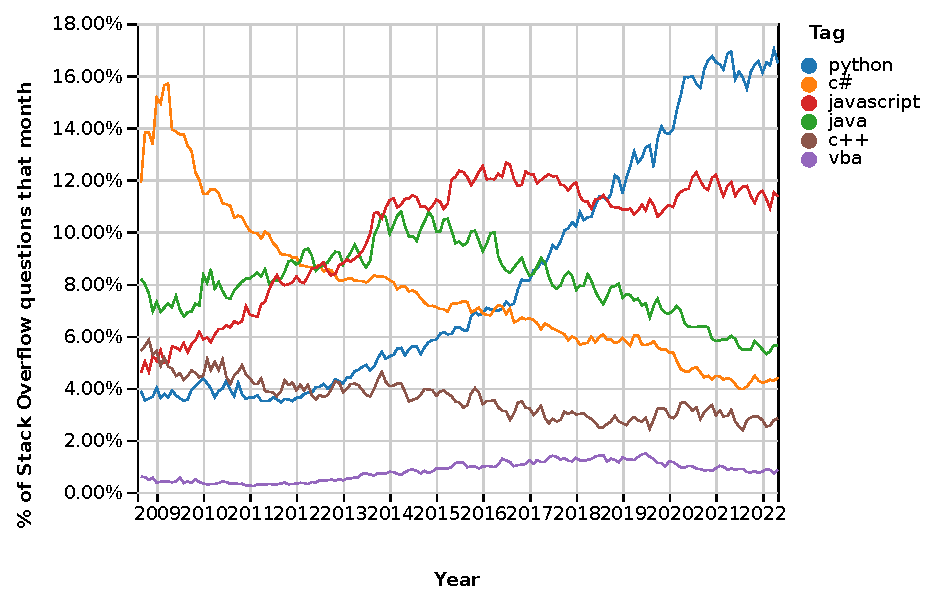
\includegraphics[width=\textwidth]{TCC_Renda/figuras/Graph1.eps}
    \fonte{\cite{StackOverflow}2009-2022}
\end{figure}

\subsection{Pandas}\label{sec:Pandas}

\par Segundo \textcite{mckinney2019} ao utilizar a ferramenta Pandas é oferecido várias estruturas para dados de alto nível e funções, o mais importante é ele ser um dado estruturado ou tabulado de forma fácil e expressiva.
%---------------------REVER---------------------------------
\par Pandas teve seu início de funcionamento a partir do ano de 2010, pandas vem ajudando projetistas e programadores de Python fazendo que seja um ambiente mais eficaz para a análise de dados.
\par O modelo que iremos utilizar nesse trabalho/projeto será o DataFrame, utilizado para estruturar dados e tabular, orientação de colunas, com rótulos (\textit\textbf{lábels}) tanto para linhas quanto para colunas e também foi utilizado Series, como um objeto array unidimensional (exemplo seria um rótulo).
%---------------------REVER---------------------------------
\par A combinação das ideias de alto processamento de \textit{arrays} utilizado no Numpy é utilizado no Pandas só que de forma mais flexíveis para ser fácil a manipulação dos dados nas planilhas de bancos de dados relacionados, um exemplo seria o SQL.
\par Pandas também disponibiliza muitas funcionalidades sofisticadas de formatação, manipulação de dados, agregações e seleções de subconjuntos de dados. Como por exemplo a manipulação de dados na analise de dados e sua limpeza e preparação para a utilização final em contas e afins.
\par Algumas funcionalidades citadas por \textsc{\cite[p.12]{mckinney2019}} seriam:

\begin{citacao}
        \par - Estruturas de dados com eixos nomeados, com suporte para alinhamento automático ou explícito de dados – isso evita erros comuns resultantes de dados desalinhados e possibilita trabalhar com dados indexados de modo diferente, provenientes de origens distintas;
        \par - Funcionalidade para séries temporais integradas;
        Mesmas estruturas de dados para lidar com séries de dados tanto temporais quanto não temporais;
        \par - Operações aritméticas e reduções que preservem metadados;
        \par - Tratamento flexível para dados ausentes;
        \par - Combinações (\textit{merge}) e outras operações relacionais que se encontram em bancos de dados populares (baseados em SQL, por exemplo).
\end{citacao}

\subsection{Numpy}\label{sec:Numpy}
A biblioteca Numpy como é dito por \textcite{mckinney2019}, é uma ferramenta que oferece o código aglutinador utilizado para estruturas de dados, como por exemplo para algorítimos e é utilizado para várias aplicações com uso de números(dados numéricos).
\par Dentro da própria ferramenta podemos encontrar os recursos:

\begin{itemize}
    \item Utilização de Arrays multidimensional chamando \textit{ndarray} para ser mais rápido e de maior eficiência;
    \item Contém funcionalidade de multiprocessamento de informação de dados em várias arrays ao mesmo tempo e/ou em uma única;
    \item Contém a ferramenta de leitura e gravura de conjuntos de dados de acordo com a array no disco;
    \item operações de álgebra linear, transformadas de Fourier e geração de números aleatórios;
    \item Utiliza uma API C já treinada tendo sua permissão de utilização de outras linguagem no mesmo código como por exemplo C ou C++, para que tenham permissões de acesso nas estruturas de dados e outros processamentos de dados feito pelo \textit{Numpy}
\end{itemize}
%---------------------REVER---------------------------------
\par De forma não exclusiva os processamentos ágeis de \textit{arrays} dentro do próprio NumPy para acrescentar ao \textit{Python}, como citado nas funcionalidades, ele tem sua maior disponibilidade em análise de dados em forma de contêiner, sendo assim possível que todo dado analisado por ele no código possa ser passado para outro programa,algoritmo, em forma de biblioteca. Focando em dados numéricos, as arrays do \textit{Numpy} tem sua maior eficiência em armazenamento e manipulação de dados em comparação a outras ferramentas que funcionam em forma de \textit{built-in} (embutidas) pelo Python.
Por conta dessa funcionalidade, os dados que vierem de dados de baixo nível, como C e Fortran, podem ser utilizados e operar em uma \textit{array} do \textit{NumPy} sem que ela seja copiado os dados de outra representação da memória.
%---------------------REVER---------------------------------

\par Fazendo assim que as funcionalidades do próprio numpy em forma de processamento numérico não são acusadas pelo \textit{Python}e assim as estruturas do \textit{Numpy} podem ser utilizados como principais ou tem sua meta uma de comunicar com outros sistema de uma forma mais suave com a utilização do \textit{NumPy}.






\subsection{PyMuPDF}\label{sec:Fitz}

\par Ao se utilizar a ferramenta-modulo Fitz proveniente da biblioteca por por PyMuPDF e disponibilizado por \textcite{MUPDF}, é possível que possa puxar valores de planilhas do Excel e assim podendo ser colocados em seu código de forma estruturada e também podendo com isso utilizar em bases com grandes quantidades de dados.
\par Com a ferramenta PyMuPDF podem ser acessados também arquivos com as extensões ".pdf" “.xps”, “.oxps”, “.cbz”, “.fb2” or “.epub”.
\par Ferramenta disponível tanto para Mac quanto Windowns e Linux com Python.
\par Com seu fácil manuseio e de forma mais simples, utilizando scripts que podem ser configurados de outras linguagens como por exemplo C e C++, sendo assim editável as instancias que irá puxar da planilha em si.
\par Podendo extrair fotos, cores, links e compressões de página, e assim deixando o dado o mais "mastigado" possível para o funcionamento do código em geral.

\subsection{DataFrame}\label{sec:dataframe}

\par De acordo com \textcite{Petrou2017-no} todo dado em um disco de memória é tornado em um \textit{DataFrame} usando apenas uma variável que está disponível na linguagem Pandas,descrito em \autoref{sec:Pandas}, o comando em questão seria \textit{"pandas.DataFrame()"} sendo ela uma função. A saída de todas as colunas e o índex estariam em negrito deixando em um formato de melhor leitura para o usuário. Durante essa conversão os termos "\textit{Index Label}" e "\textit{Collumn Name}"  são referidos ao número individual dos membros do índice e da coluna em questão.
\begin{figure}[!]
    \caption{\label{fig:Fig_2}Estrutura de DataFrame.}
    \begin{center}
    \resizebox{\columnwidth}{!}{
    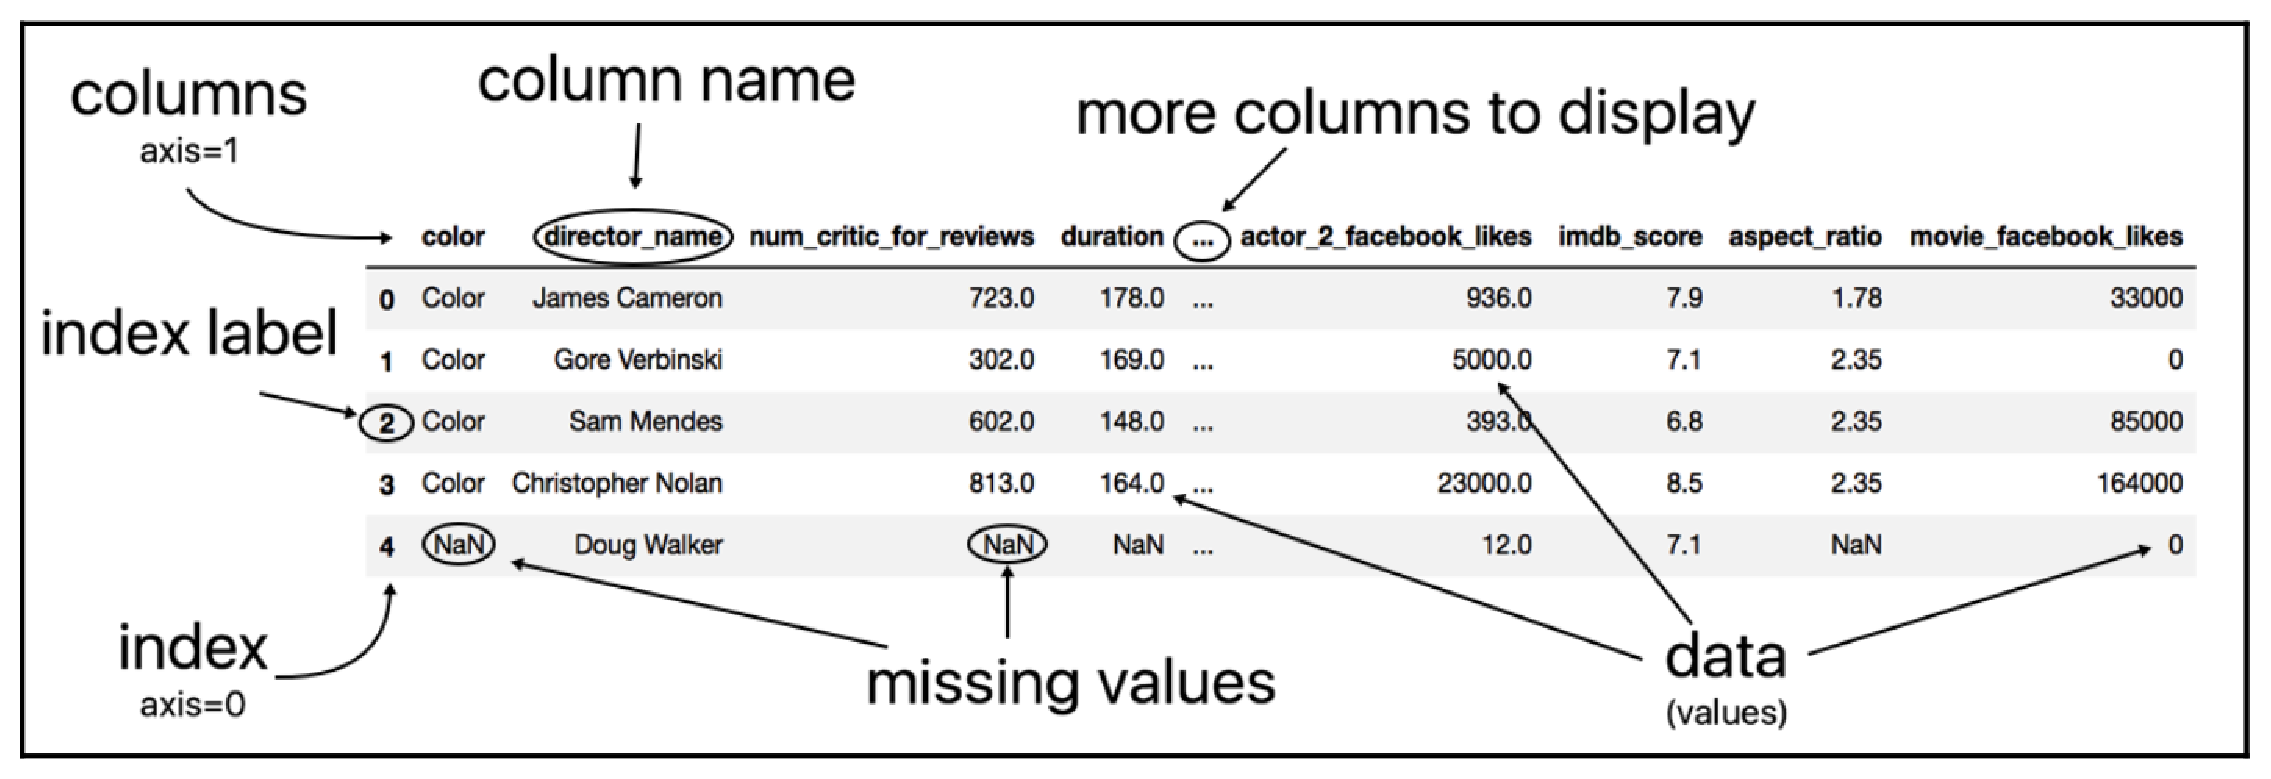
\includegraphics[width=\textwidth]{TCC_Renda/figuras/Dataframe.eps}
    }\end{center}
	\fonte{\cite[P.17]{Petrou2017-no}}
\end{figure}
\par O termo \textit{index} é referido à todos os rótulos de indicies como um todo, assim como o termo colunas se refere a todas as colunas
nomes como um todo.

\par A coluna do índice tem uma serventia em particular, e essa tem a função de prover rótulos para as colunas e as informações que entraram ao \textit{DataFrame}. Esses rótulos permitem que de forma direta e mais simples, possam ser acessados esses dados e sendo ele de diferentes locais em que o dado for colocado.

\par Quando vários tipos de \textit{DataFrames} são combinados esses indicies são alinhados primeiramente antes de qual quer tipo de cálculo seja feito. Disse \cite{Petrou2017-no} que,"Coletivamente, as colunas e o índice são conhecidos como os eixos."

\par Dado os Dados em que o \textit{DataFrame} sempre estão em forte regulares e também são componentes totalmente independentes tanto das colunas quanto do índice.
Já na ferramenta Pandas é utilizado o NaN(\textit{Not a Number}) para ser utilizado a representação dos valores que não são encontrados pela busca de dados.
\par Olhando para \autoref{fig:Fig_2} , podemos observar que a coluna de cores tem apenas valores de forma (\textit{"String"}), é utilizado o NaN para representar um valor ausente.

	\begin{figure}[ht]
    \caption{\label{fig:Fig_4}Fluxograma do trabalho.}
    \begin{center}
    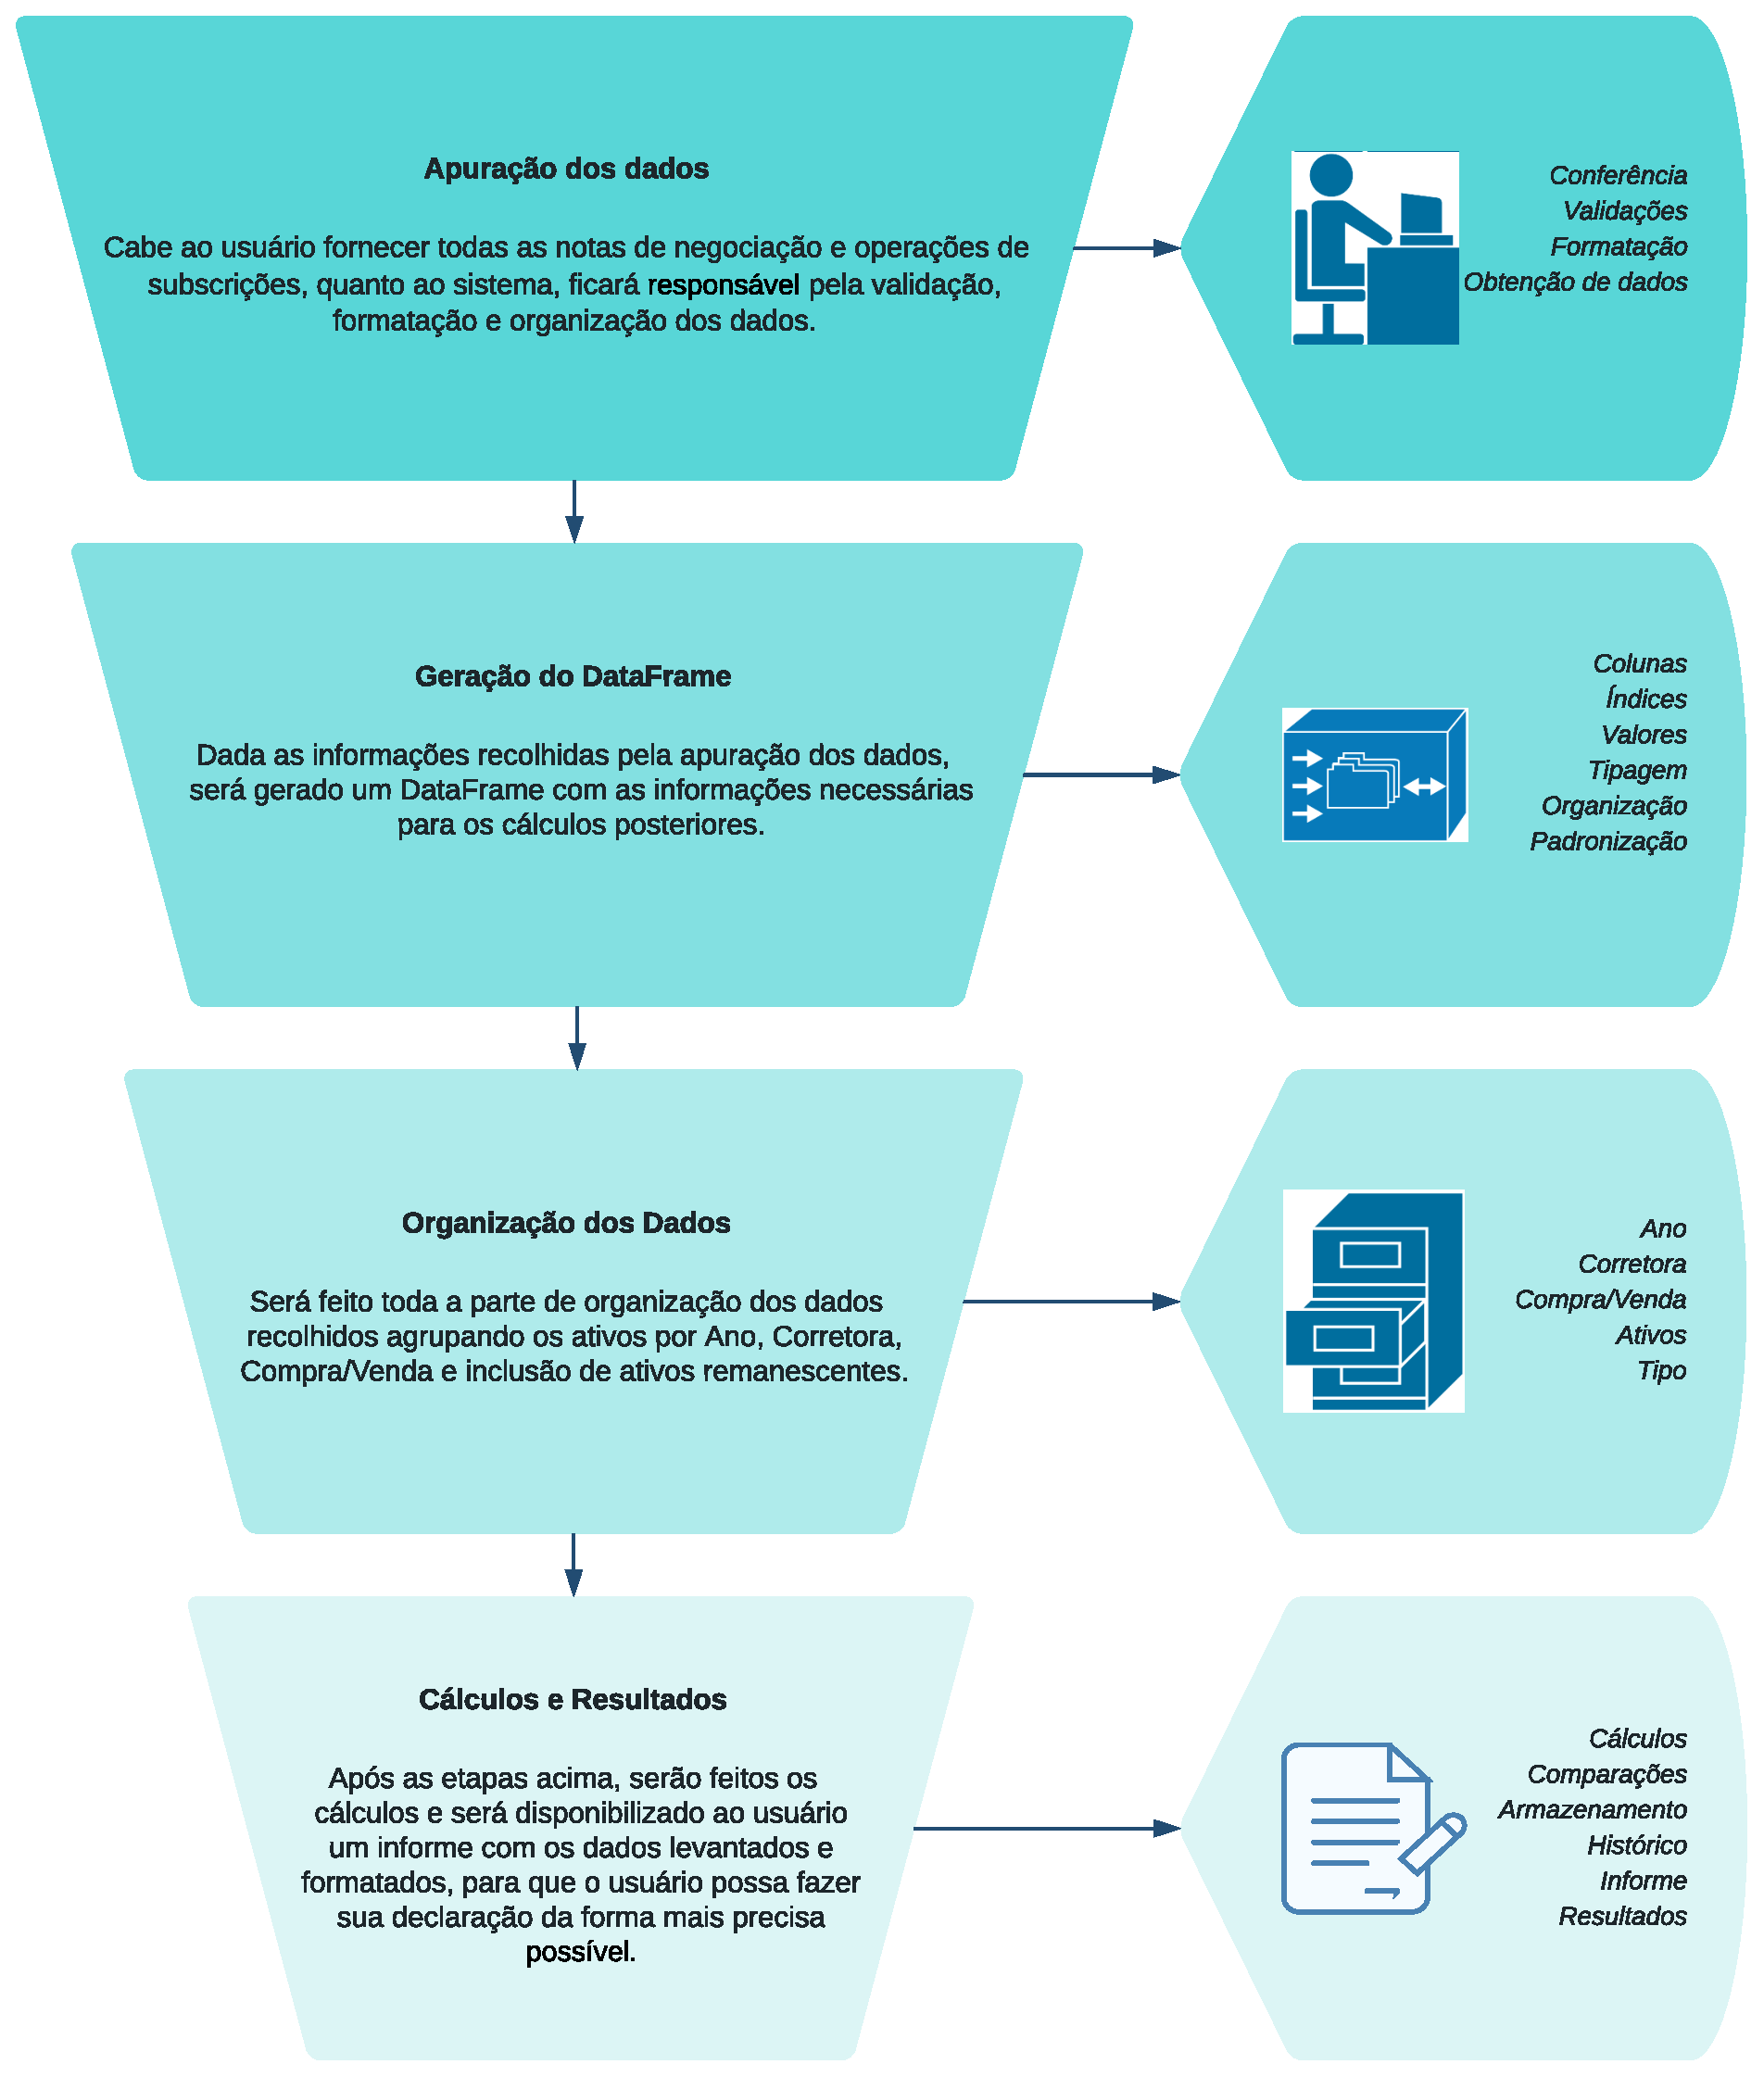
\includegraphics[scale=0.45]{TCC_Renda/figuras/TCC Fluxograma V5.eps}
    \end{center}
	\fonte{Autores do trabalho}
    \end{figure}
	

	

	% 4 - Desenvolvimento 	- Conclusão
	
% ----------------------------------------------------------


 \section{\textbf{Apuração dos dados}}%\label{cap:desenvolvimento}
 
% ----------------------------------------------------------
\par Nesta etapa de apuração seguiremos as chamadas da função destacada na \autoref{fig:Fig_3}, de inicio o usuário precisaria fornecer todos os dados necessários, para que seja possível a análise correta pelo sistema.

\begin{figure}[ht]
    \caption{\label{fig:Fig_3}Função Iniciar levantamento.}
    \begin{center}
    \resizebox{\columnwidth}{!}{
    \includegraphics[scale = 0.745]{TCC_Renda/figuras/Funcao preencher.eps}
    }\end{center}
	\fonte{Autores do trabalho}
\end{figure}

\par Foi escolhido esse método de coleta por conta da própria segurança e confiabilidade que o usuário terá, sendo ele mesmo encargo de sua responsabilidade, e desligado de quaisquer bancos de dados online, onde seus dados não sairão de sua máquina durante a utilização da aplicação.


\par Após o fornecimento dos dados o sistema irá ler os arquivos que estão em formatação PDF e Excel, em seus respectivos diretório.

\par Com os dados computados é necessário fazer as formatações necessárias, para formalizar as informações para as quais serão utilizados durante os cálculos futuros.

\par Após toda a formatação ele irá fazer a limpeza dos dados para que haja uma estruturação de melhor qualidade e re-colocando em variáveis suas respectivas posições assim como, cada um tem sua cadeira e cada um tem seu local correto de informação, claro com base na formatação como dito a cima no último parágrafo.

\subsection{Geração do DataFrame}

\par A geração do DataFrame  tera sua formatação com base nos dados extraídos da apuração dos dados, com eles os dados descritos na \autoref{tab:Tab_1}:



\par Com dada lista de negócios adquiridos de cada arquivo computado os valores recolhidos passam para um vetor, sendo assim cada posição do vetor equivale a uma coluna do DataFrame, é feito um \textit{loop} para o preenchimento do dataframe de acordo com a quantidade de negócios realizados em cada nota de negociação. É gerado um Dataframe para cada ano, relacionando todos os negócios feitos naquele ano, para servir de comparativo ao do ano antecessor de suas negociações.

\subsubsection{\textbf{Formatação DataFrame}}


\par Durante a formatação de dados será realizado a primeira filtragem de separação de dados sendo ela em relação ao ano do ativo que foi negociado, isso por conta dos cálculos que são feitos de forma progressiva com base na data de Compra e data de Venda de cada ativo.
\par Todos os índices são setados em ordem crescente, valores de texto que representam números serão formatados, alterando virgulas para pontos, pois a linguagem utilizada não permite a sintaxe de valores com virgulas.
\par Os valores em \textit{String} (formato utilizado para textos) são passados para formato \textit{Float}(formato utilizado para números).

\begin{table}[ht]
\ABNTEXfontereduzida
\caption{\label{tab:Tab_1}Estrutura do DataFrame utilizado molde das notas de negociação.}
\resizebox{\columnwidth}{!}{
\begin{tabular}{|l|l|l|l|l|l|l|}
\hline
Data & Entrada/Saída & Instituição & Produto & Quantidade & Preço unitário & Valor da Operação \\ \hline
\end{tabular}%
}
%\fonte{XP Investimentos 2020/2021.}
\end{table}

\par Para identificação de cada ativo, precisamos do código de negociação disponível no diretório /\textit{info}/ no arquivo de base de dados Excel.
	
\par O código de negociação é implementado no dataframe, de acordo com cada tipo, o código pode ser de formato prioritário ou ordinária, sendo isso uma função de alta importância para a organização dos dados, a ação prioritária teria o valor concatenado final igual a "4", já a ordinária seria o valor concatenado de final "3". Por fim as datas tem sua formatação geradas em formato,\textit{datetime}, que por sua vez tem a permissão para comparações de forma booleana, um podendo comparar com a outra para assim ter o resultado se uma é maior que a outra, e assim terminando a formatação básica do dataframe.

\subsection{Ativos remanescentes}

\par Caso houver ativos remanescentes do ano anterior ao ano a ser calculado no \autoref{sec:carteira} será necessário fazer uma concatenação de valores do DataFrame da carteira, com os valores a serem calculados do DataFrame do ano em questão.
%----------------------------------------------------------
\subsection{\textbf{Agrupamento de Dados}}

\par Nesta etapa visando separar o dataframe para ser possível efetuar futuros cálculos, será feito um agrupamento dos ativos por corretora. Também agruparemos as operações de compra e venda em diferentes dataframes. Também será definido o tipo de cada ativo, sendo ele uma ação ou um fundo imobiliário.



\par Os ativos serão separados por valores únicos, assim será possível iterar de forma individual em cima de todas as negociações referentes ao seu código de negociação, pois os cálculos serão realizados de forma separada para cada ativo.

\subsubsection{\textbf{Agrupamento por corretora}}

\par As operações feitas em uma corretora "X" não podem interferir nos cálculos de uma corretora de nome "Y", então nesta fase o sistema faz o devido agrupamento. 
 
\subsubsection{\textbf{Agrupamento por compra e venda}}

\par Caso a pessoa teve uma compra de 100 ações no começo do ano e por acaso comprou mais 100 durante o período do ano, é preciso calcular o preço médio das ações adquiridas, porem é necessário verificar se houve uma venda anterior a compra seguinte, que tenha alterado a posição inicial de 100 ações, isso alteraria os valores do preço médio calculado. Por isso foi dividido entre dataframes diferentes, sendo eles um de Compra outro de Venda, para assim facilitar a visibilidade das operações durante o período a ser consultado.



\textbf{\subsection{Cálculos finais}}\label{sec:carteira}


\par Neste ponto, de acordo com a \autoref{fig:Fig_5} serão realizados os cálculos de lucro, posição e preço médio dos ativos que estão sendo processados. 

\par Para o cálculo do preço médio, será feito uma somatória dos valores de compra e quantidade individualmente para todas as compras com data inferior há última data de venda, 
com isso podemos obter e calcular o preço médio, dividindo o total de compra pela quantidade total de compra.


\par Para ser feito o cálculo do lucro, será subtraído do valor resultante da venda, o valor obtido pela multiplicação do preço médio e quantidade de venda em relação a data.

\begin{figure}[h]
    \caption{\label{fig:Fig_5}Função preço médio, posição e lucro.}
    \begin{center}
    \includegraphics[width=\textwidth]{TCC_Renda/figuras/defcalc.eps}
    \fonte{Autores do trabalho}
    \end{center}
\end{figure}

\par Já para o cálculo da posição, caso haja vendas há serem calculadas será subtraído a somatória da quantidade de compra até o momento da data de venda, caso existam compras posteriores em relação última data de venda simplesmente será feita a somatória.

\section{\textbf{Resultados obtidos}}\label{sec:resultado}

\par Como demonstrado na \autoref{fig:Fig_6} o informe final foi gerado com sucesso, seguindo os valores alcançados pelas etapas anteriores. O informe está composto entre os principais campos que o usuário precisará para que seja possível a declaração de seu imposto de renda.

\par A estrutura foi dividida seguindo os códigos presentes no aplicativo de imposto de renda IRPF  \textcite{IRPF2022}, direcionando o usuário á informação correta de seus investimentos. O valor do "Ano" do documento será dinamicamente alterado conforme o ano do exercício da declaração. 

\par O valor do campo "Empresa" está sendo buscado dentro da nossa base local, assim como o valor do campo CNPJ. Já os demais valores referentes aos demais campos são obtidos através dos DataFrames construídos durante o processo.

\par Em casos em que o usuário possua uma mesma ação em diferentes corretoras o informe reunirá as informações em um só bloco demonstrativo e por fim terá um campo "TOTAL", com a somatória dos valores de posição e situação entre as duas corretoras.

\section{\textbf{Considerações finais}}
\addcontentsline{toc}{section}{Considerações finais}

Foi possível alcançar o resultado esperado durante a produção deste trabalho, que por sua vez é ajudar diversos investidores, simplificando sua tarefa de fazer o lançamento do seu imposto de renda anual, que para muitos é de difícil compreensão, podendo causar muita confusão.
Com os resultados organizados e calculados de forma autômata, diminuímos os problemas encontrados por todos os tipos de investidores, fornecendo a eles um controle do que de fato possuem em seu patrimonio para que possam transparece-lo ao governo de forma legitima, e que no futuro não se deparem com problemas com a receita federal.

 Deve-se considerar a constante atualização da base de dados local utilizada no trabalho, pois diversas empresas passam a participar da bolsa abrindo o seu  patrimonio, essas informações são importantes para construção do informe final.
Outra consideração a ser feita, os códigos de referencia do bem e ficha de declaração utilizados pelo aplicativo do governo podem ser alterados anualmente e devem ser atualizados conforme as orientações apresentadas pelo aplicativo do governo, em relação ao ano de exercício em questão.

Considerando que, não foram encontrados trabalhos de referência no mesmo âmbito ao tema utilizado, teve-se uma dificuldade para reunir todo o conhecimento necessário em que foi baseado o trabalho. Tendo em conta que sua base se dá em cima da linguagem Python, foi possível a criação de Dataframes que ajudaram na obtenção dos dados tanto eles em grande, quanto em pequena escala. Também para que futuramente tenha um melhor desenvolvimento deste trabalho, pode-se acrescentar outros tipos de investimentos, e também a adaptação do código para diferentes modelos de notas de negociação, permitindo atingir cada vez mais pessoas que necessitariam exercer essas obrigações como cidadão.

Mesmo sabendo que ainda não  chegamos ao resultado esperado do trabalho, por conta tanto de fatores externos, sendo eles a que não atende a todos os tipos de formulários, dito isso, o trabalho irá ficar em aberto para que possa ser implementado futuramente novas ferramentas e interfaces que atendam a máxima necessidade dos usuários.

%\section{Exposição do tema ou matéria}

%É a parte principal e mais extensa do trabalho. 
%Deve apresentar a fundamentação teórica, a metodologia, os resultados e a discussão. Divide-se em seções e subseções conforme a NBR 6024 \cite{NBR6024:2012}.
	

	% ----------------------------------------------------------

\begin{figure}[h]
    \caption{\label{fig:Fig_6}Demonstrativo final.}
    \begin{center}
    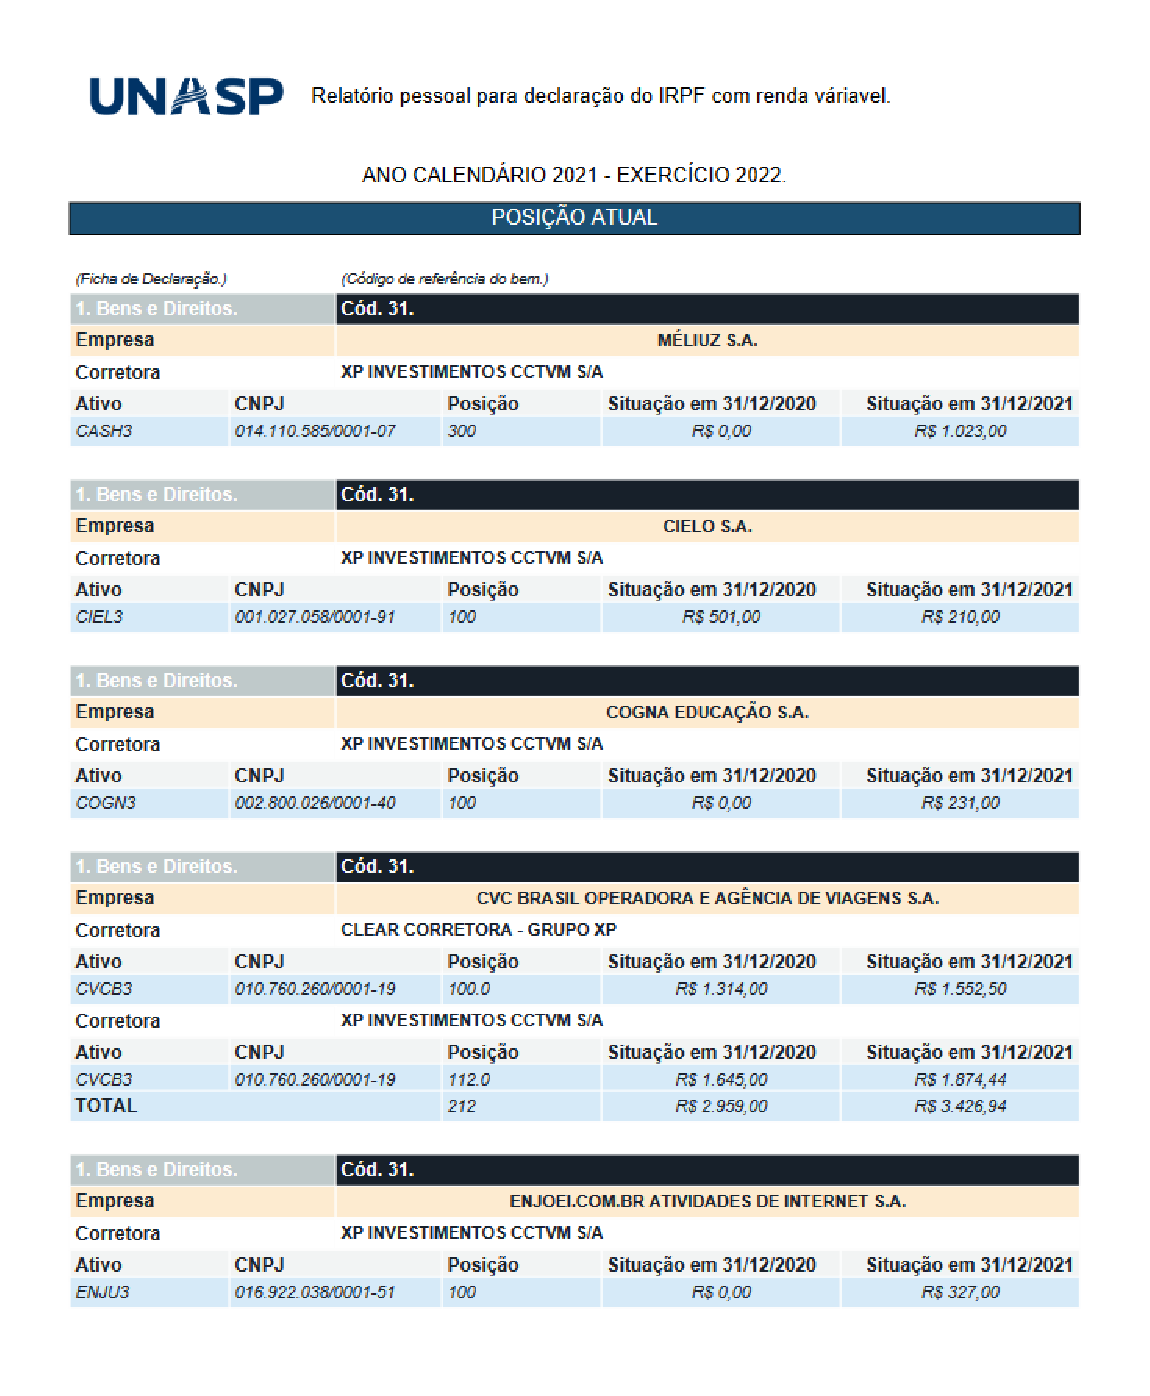
\includegraphics[width=\textwidth]{TCC_Renda/figuras/resultado final.eps}
    \fonte{Autores do trabalho}
    \end{center}
\end{figure}
% ----------------------------------------------------------

%As conclusões devem responder às questões da pesquisa, em relação aos objetivos e às hipóteses. Devem ser breves, podendo apresentar recomendações e sugestões para trabalhos futuros.
	

	% Elementos pós-textuais
	\postextual
	
	
	% Referências bibliográficas
	\begingroup
	    \printbibliography[title=REFERÊNCIAS]
	\endgroup
	
	
	
	%Reconfiguração do título para apêndices e anexos
	 \renewcommand{\ABNTEXchapterupperifneeded}[1]{#1} 
	\makeatletter
	\settocpreprocessor{chapter}{%
      \let\tempf@rtoc\f@rtoc%
      \def\f@rtoc{%
      \texorpdfstring{{\tempf@rtoc}}{\tempf@rtoc}}%
      }
    \makeatother
	
%tire o "%" se houver esta função em seu trabalho!!!

% Apêndices
%  \begin{apendicesenv}
%   \partapendices* 
%	% ----------------------------------------------------------
\chapter{Descrição}   %Apenas a primeira letra deve ser maiúscula
% ----------------------------------------------------------

%Textos elaborados pelo autor, a fim de completar a sua argumentação. Deve ser precedido da palavra APÊNDICE, identificada por letras maiúsculas consecutivas, travessão e pelo respectivo título. Utilizam-se letras maiúsculas dobradas quando esgotadas as letras do alfabeto. 

%\end{apendicesenv}

% Anexos
%\begin{anexosenv}
  %\partanexos*
%   % ----------------------------------------------------------
\chapter{Descrição}   %Apenas a primeira letra deve ser maiúscula
% ----------------------------------------------------------

%São documentos não elaborados pelo autor que servem como fundamentação (mapas, leis, estatutos). Deve ser precedido da palavra ANEXO, identificada por letras maiúsculas consecutivas, travessão e pelo respectivo título. Utilizam-se letras maiúsculas dobradas quando esgotadas as letras do alfabeto. 

%\end{anexosenv}

\end{document}